\documentclass[12pt, a4paper]{article}
% --- Packages ---
\usepackage[utf8]{inputenc}
\usepackage[T1]{fontenc}
\usepackage[french]{babel}
\usepackage{graphicx} % Make sure this is here for images
\usepackage{booktabs}
\usepackage{amsmath}
\usepackage{geometry}
\usepackage{array}
\usepackage{enumitem}
\usepackage{hyperref}
\usepackage{xcolor}
\usepackage{titlesec}
\usepackage{lmodern}
\usepackage{microtype}
\usepackage{fancyhdr}
\usepackage{listings} % Added for code/JSON display
\usepackage[scaled=0.85]{beramono} % Added for a nicer monospaced font

% --- Font Configuration ---
% --- Color Definitions ---
\definecolor{primary}{RGB}{0,51,102}
\definecolor{secondary}{RGB}{102,102,153}
\definecolor{accent}{RGB}{204,0,0}
\definecolor{codegray}{rgb}{0.5,0.5,0.5}
\definecolor{codepurple}{rgb}{0.58,0,0.82}
\definecolor{codeblue}{rgb}{0,0,0.9}
\definecolor{codegreen}{rgb}{0.1,0.6,0.1} % Darker green for comments

% --- Page Geometry ---
\geometry{
  a4paper,
  left=2.5cm,
  right=2.5cm,
  top=2.5cm,
  bottom=2.5cm,
  headheight=15pt
}
% --- Header/Footer Setup ---
\pagestyle{fancy}
\fancyhf{}
\fancyhead[L]{\small Rapport de Stage - Semaine 4 - Jour 6} % Updated
\fancyhead[R]{\small Zakaria el Khaldi}
\fancyfoot[C]{\thepage}
\renewcommand{\headrulewidth}{0.4pt}
\renewcommand{\footrulewidth}{0.4pt}
% --- Title Formatting ---
\titleformat{\section}
  {\normalfont\Large\bfseries\color{primary}}
  {\thesection}{1em}{}
\titleformat{\subsection}
  {\normalfont\large\bfseries\color{secondary}}
  {\thesubsection}{1em}{}
\titleformat{\subsubsection}
  {\normalfont\normalsize\bfseries\color{accent}}
  {\thesubsubsection}{1em}{}
% --- List Formatting ---
\setlist[itemize]{leftmargin=*, nosep}
\setlist[enumerate]{leftmargin=*, nosep}
% --- Hyperlink Setup ---
\hypersetup{
  colorlinks=true,
  linkcolor=primary,
  urlcolor=secondary,
  citecolor=accent
}

% --- Listings Setup for JSON ---
\lstdefinestyle{json}{
    language=json,
    basicstyle=\ttfamily\footnotesize,
    numbers=left,
    numberstyle=\tiny\color{codegray},
    stepnumber=1,
    numbersep=5pt,
    backgroundcolor=\color{white!95!black}, % Very light gray background
    showspaces=false,
    showstringspaces=false,
    showtabs=false,
    frame=tb, % Top and bottom frame
    framextopmargin=3pt,
    framexbottommargin=3pt,
    rulecolor=\color{black!30!white},
    tabsize=2,
    captionpos=b,
    breaklines=true,
    breakatwhitespace=false,
    stringstyle=\color{codepurple},
    commentstyle=\color{codegreen},
    keywordstyle=\color{codeblue}, % For true, false, null
    morestring=[b]",
    literate=
     *{0}{{{\color{codeblue}0}}}{1}
      {1}{{{\color{codeblue}1}}}{1}
      {2}{{{\color{codeblue}2}}}{1}
      {3}{{{\color{codeblue}3}}}{1}
      {4}{{{\color{codeblue}4}}}{1}
      {5}{{{\color{codeblue}5}}}{1}
      {6}{{{\color{codeblue}6}}}{1}
      {7}{{{\color{codeblue}7}}}{1}
      {8}{{{\color{codeblue}8}}}{1}
      {9}{{{\color{codeblue}9}}}{1}
      {:}{{{\color{black}:}}}{1}
      {\{}{{{\color{black}{\{}}}}{1}
      {\}}{{{\color{black}{\}}}}}{1}
      {[}{{{\color{black}{[}}}}{1}
}


% --- Title Page Information ---
\title{\Huge\bfseries\color{primary} Rapport de Stage \\ 
      \Large Semaine 4 - Jour 6 : Finalisation des Interfaces d'Authentification et Préparation Backend} % Updated title
\author{\Large Zakaria el Khaldi}
\date{\large Le 2 Juin 2025} % Updated date for Day 6, Week 4 (Saturday, document dated for next working day or submission)

% --- Document Start ---
\begin{document}
% --- Cover Page ---
\begin{titlepage}
  \centering
  \vspace*{\stretch{0.5}}
  {\Huge\bfseries\color{primary} Rapport de Stage \par}
  \vspace{1cm}
  {\Large\itshape Semaine 4 - Jour 6 : Interfaces d'Accès Utilisateur et Expérimentation Nginx\par} % Updated title
  \vspace{2cm}
  
  \vspace{2cm}
  {\Large Zakaria el Khaldi\par}
  \vfill
  {\large Le 31 Mai 2025\par} % Date of activity day (Saturday)
  \vspace*{\stretch{1}}
\end{titlepage}

% --- Table of Contents ---
\tableofcontents
\thispagestyle{empty}
\newpage

% --- Introduction ---
\section{Introduction}
\thispagestyle{fancy}
Ce sixième et dernier jour de la quatrième semaine de stage a été consacré à la finalisation des interfaces d'authentification de la plateforme LearnExpert, un composant crucial pour l'accès utilisateur. Suite à cela, l'attention s'est portée sur l'expérimentation de Nginx en tant que passerelle API (API Gateway) et répartiteur de charge (load balancer), en préparation du développement backend prévu pour la semaine suivante. Ces étapes sont fondamentales pour établir une architecture robuste et évolutive.

% --- Day's Accomplishments ---
\section{Activités du Jour (Samedi 31 Mai 2025)} % Updated day and date

\subsection{Finalisation des Interfaces d'Authentification}
Le développement des différentes pages du flux d'authentification a été complété, garantissant une expérience utilisateur cohérente et sécurisée pour l'accès à la plateforme.

\subsubsection{Processus de Création de Compte}
L'interface de création de compte a été finalisée. Elle guide l'utilisateur à travers plusieurs étapes : la saisie des informations de base (nom complet, adresse e-mail) (Voir Figure \ref{fig:signup_basic_info}), puis la configuration de la sécurité du compte avec la définition et la confirmation du mot de passe, incluant des indicateurs de force du mot de passe et des critères de validation. (Voir Figure \ref{fig:signup_security}).

\begin{figure}[htbp]
  \centering
  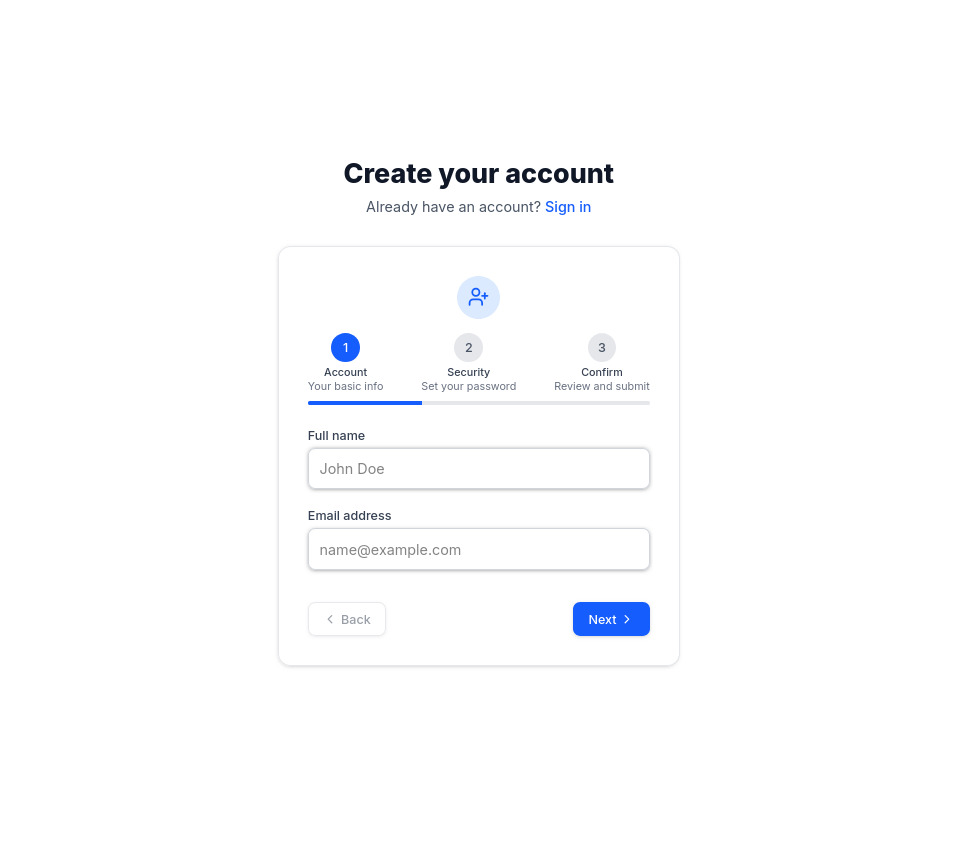
\includegraphics[width=0.6\textwidth]{etap1.jpeg} 
  \caption{Interface de création de compte - Étape 1 : Informations de base.}
  \label{fig:signup_basic_info}
\end{figure}

\begin{figure}[htbp]
  \centering
  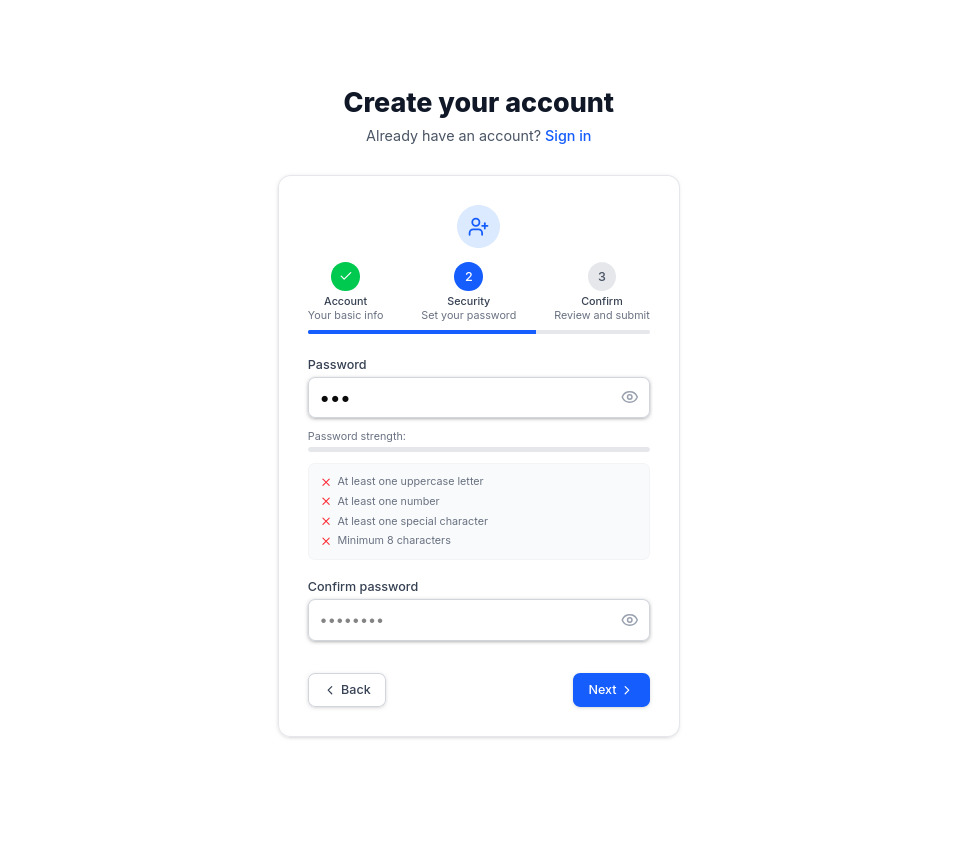
\includegraphics[width=0.6\textwidth]{etap2.jpeg} 
  \caption{Interface de création de compte - Étape 2 : Configuration du mot de passe.}
  \label{fig:signup_security}
\end{figure}

\subsubsection{Interface de Connexion (Sign In)}
La page de connexion a été implémentée, permettant aux utilisateurs existants d'accéder à leur compte via leur adresse e-mail et mot de passe. Des options pour se souvenir de l'utilisateur et des liens vers la création de compte et la récupération de mot de passe sont également présents, ainsi que des options de connexion via des services tiers (Google, GitHub, Twitter). (Voir Figure \ref{fig:signin_page}).

\begin{figure}[htbp]
  \centering
  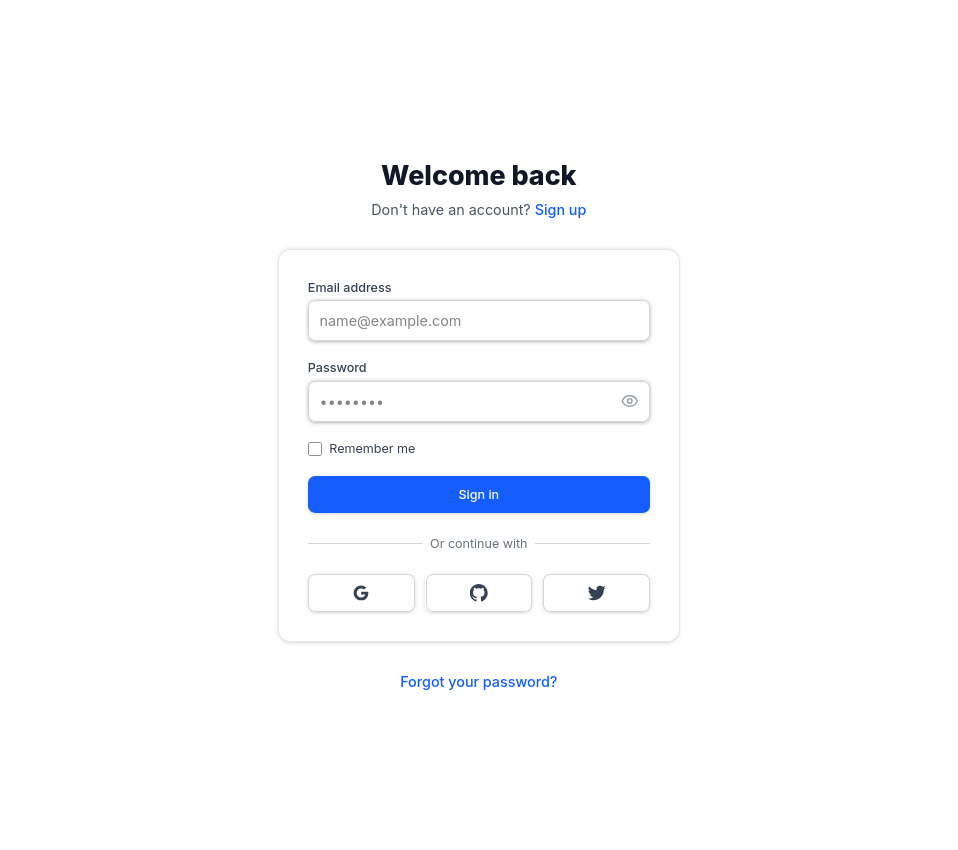
\includegraphics[width=0.6\textwidth]{login.jpeg} 
  \caption{Interface de connexion à la plateforme.}
  \label{fig:signin_page}
\end{figure}

\subsubsection{Processus de Récupération de Mot de Passe}
Le flux de récupération de mot de passe a été mis en place. Il commence par la saisie de l'adresse e-mail associée au compte (Voir Figure \ref{fig:forgot_password_email}), suivie d'une page de confirmation indiquant qu'un lien de réinitialisation a été envoyé. (Voir Figure \ref{fig:forgot_password_confirmation}).

\begin{figure}[htbp]
  \centering
  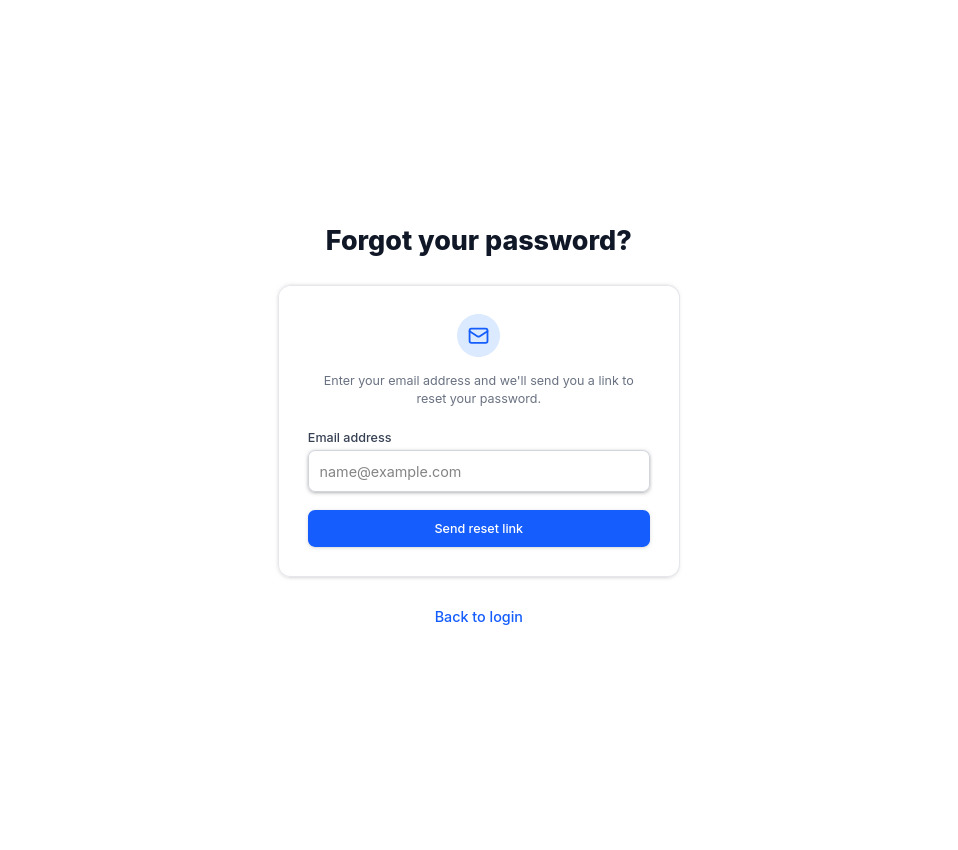
\includegraphics[width=0.6\textwidth]{reset.jpeg} 
  \caption{Interface de récupération de mot de passe - Saisie de l'email.}
  \label{fig:forgot_password_email}
\end{figure}

\begin{figure}[htbp]
  \centering
  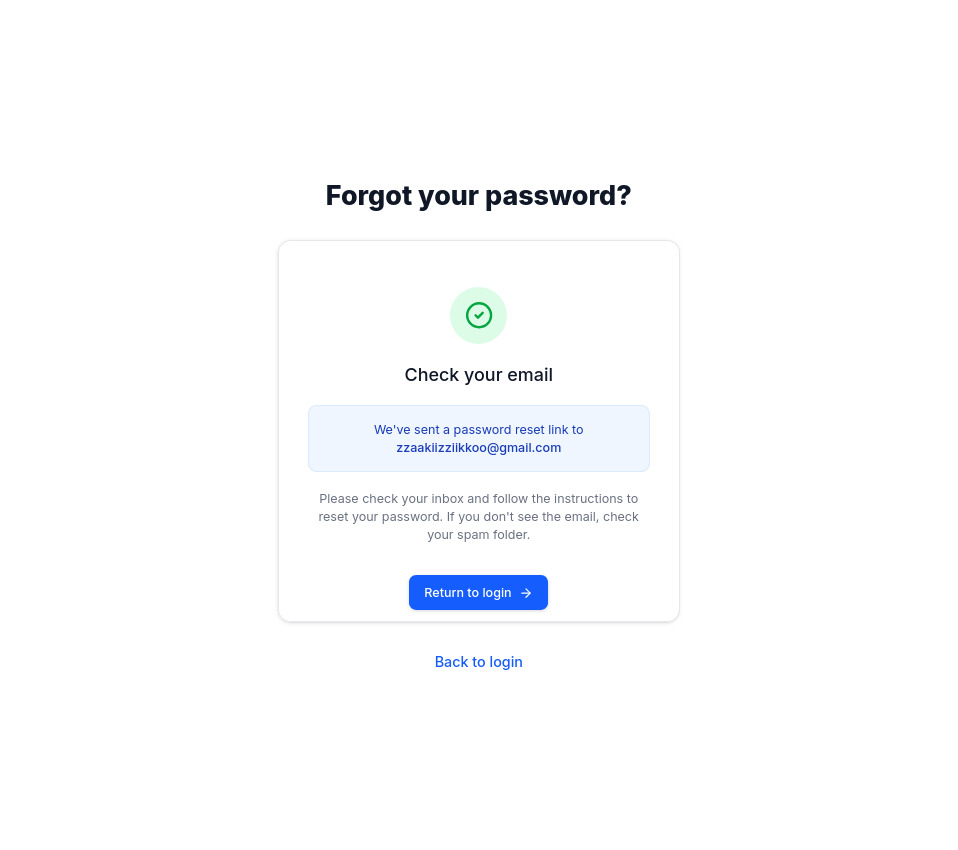
\includegraphics[width=0.6\textwidth]{sended.jpeg} 
  \caption{Interface de récupération de mot de passe - Confirmation d'envoi.}
  \label{fig:forgot_password_confirmation}
\end{figure}

\newpage

\subsection{Expérimentation avec Nginx comme API Gateway et Load Balancer}
Une fois les interfaces d'authentification complétées, la journée a été consacrée à l'exploration et à l'expérimentation de Nginx. L'objectif était de :
\begin{itemize}
    \item Comprendre sa configuration en tant que passerelle API pour gérer les requêtes entrantes et les router vers les futurs microservices.
    \item Tester ses capacités de répartition de charge (load balancing) pour assurer la scalabilité et la haute disponibilité des services backend.
    \item Évaluer son intégration dans l'architecture globale de la plateforme en vue du développement backend.
\end{itemize}
Cette phase d'expérimentation est cruciale pour définir l'infrastructure qui supportera les services de la plateforme.



\subsection{Planification pour la Semaine Suivante (Semaine 5)}
Pour la semaine prochaine, les activités principales prévues sont :
\begin{itemize}
  \item Démarrer activement le développement backend, en adoptant une architecture microservices.
  \item Configurer et mettre en place la passerelle API Nginx de manière plus formelle, basée sur les apprentissages de l'expérimentation.
  \item Commencer le développement du service IAM (Identity and Access Management), qui sera responsable de la gestion des utilisateurs, de l'authentification, et des autorisations au sein de la plateforme. Ce service sera le premier microservice clé de l'architecture.
\end{itemize}

\section{Conclusion}
Cette sixième journée de la quatrième semaine de stage a permis de clore le cycle de développement des interfaces d'authentification, essentielles pour l'expérience utilisateur. L'après-midi a été productivement utilisée pour l'expérimentation de Nginx, posant ainsi les bases techniques pour l'infrastructure backend. La semaine 4 s'achève sur des réalisations significatives en matière d'UI et une préparation solide pour la transition vers le développement backend et l'architecture microservices dès la semaine prochaine.

\end{document}